\section{Основная часть}
\subsection{Датасет CIFAR-10}
Набор данных, на котором проводились исследования, состоит из 60\,000 цветных изображений, размера 
32$\times$32 пикселя. Каждое изображение принадлежит одному из 10 классов, что соответствует 600 изображениям на класс. Под 
обучение отводится 50\,000 изображений. Остальные 10\,000 используются для тестирования. Объекты в классах сильно варьируются, 
например, класс <<птица>> содержит различные виды птиц, как большие так и маленькие. Кроме того, объекты классов представлены в 
различных позах и под различными углами. Особенно это проявляется среди собак и котов, которые изображены не только в различных 
позах, но иногда и частично, например, изображена только голова животного.

Датасет CIFAR-10 \cite{learningmultiple} был выбран для проведения исследований благодаря своему относительно небольшому размеру, 
который позволяет обучать глубокие нейронные сети используя GPU с памятью меньше 8\,Gb, например, в данной работе использовалась 
NVIDIA Grid K520 с 4\,Gb видеопамяти.

На момент написания работы лучший результат (state-of-the-art) на CIFAR-10 составляет 96,53\% \cite{2014arXiv1412}. Точность  
распознавания человека равна $\approx94\%$.\footnote{\url{http://karpathy.github.io/2011/04/27/manually-classifying-cifar10/}}

\begin{figure}[h]
\centering
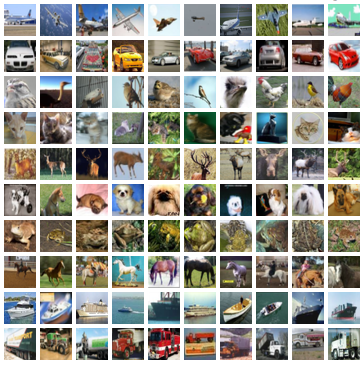
\includegraphics[width=0.5\textwidth]{cifar10}
\caption{10 случайных изображений из каждого класса CIFAR-10}
\end{figure}

\subsection{Фреймворк Caffe}
Обучение нейронных сетей проводилось с использованием фреймворка для глубокого обучения Caffe \cite{jia2014caffe}.
Изначально, фреймворк разрабатывался командой BVLC (Berkeley Vision and Learning Center), но постепенно перерос в большой 
open-source проект.\footnote{\url{https://github.com/BVLC/caffe}} На данный момент вклад в развитие Caffe внесли почти 200 
разработчиков и более 10\,000 человек оценили проект на Github.

Данный фреймворк был выбран для решения задачи по нескольким причинам:
\begin{enumerate}
    \item Простота определения моделей и методов оптимизации. Топологии нейронных сетей и алгоритмы оптимизации удобно и 
    эффективно определяются в специальных конфигурационных файлах типа Google Protocol 
    Buffers.\footnote{\url{https://developers.google.com/protocol-buffers/}} Caffe поддерживает топологии сетей в форме любых 
    ациклических графов.
    \item Модульность. Caffe позволяет легко изменять архитектуру сети под новые форматы входных данных. Кроме того, в наличии 
    имеется много слоёв и функций потерь.
    \item Скорость вычислений и эффективное использование ресурсов. Caffe заранее выделяет ровно столько памяти сколько нужно для 
    нейронной сети. Операций линейной алгебры такие как умножение, сложение и свёртка выполняются на CPU с помощью BLAS (Basic 
    Linear Algebra Subroutines). На GPU за эти операции отвечают библиотеки cuBLAS и cuDNN 
    \cite{DBLP:journals/corr/ChetlurWVCTCS14}
    \item CLI (command line interface) и интерфейсы для Python и Matlab.
\end{enumerate}

Caffe написан на языках C++, Cuda, Python. Для хранения больших объёмов данных используются базы данных 
LMDB\footnote{\url{http://symas.com/mdb/}} и LevelDB\footnote{\url{https://github.com/google/leveldb}}. Обучение нейронных сетей 
может выполняться как на CPU, так и на нескольких GPU одновременно. Фреймворк доступен для установки на Linux, Windows и OS X.

\subsection{Предварительная обработка данных}
Необработанные изображения содержат излишнюю информацию, так как смежные пиксели имеют высокую корреляцию. Поэтому прежде чем 
подавать изображения на вход нейронной сети, они были обработаны в два этапа. В начале, была произведена глобальная нормализация контраста
(global contrast normalization) изображения:
\[ \widehat{X} = \cfrac{X - \overline{X}}{\sigma},\]
где $X$ --- исходное изображение, $\overline{X}$ --- среднее значение, $\sigma$ --- стандартное отклонение.

Затем изображения были линейно трансформированы с помощью алгоритма <<ZCA whitening>> \cite{learningmultiple}.
Цель данного алгоритма сделать так, чтобы входные изображения слабо коррелировали друг с другом.

Алгоритм <<ZCA whitening>>:
\begin{lstlisting}[language=Python, frame=TB]
cov = np.dot(X.T, X) / X.shape[0] #%* Вычисляем ковариационную матрицу *)
U,S,V = np.linalg.svd(cov) #%* Находим сигнулярное разложение ковариацонной матрицы *)
Xrot = np.dot(X, U) #%* Поворачиваем входные данные *)
Xwhite = Xrot / np.sqrt(S + %*$\alpha$*)) #%* Делим на собственные числа *)
\end{lstlisting}
\vspace*{-1.4cm}
\begin{figure}[h]
    \centering
    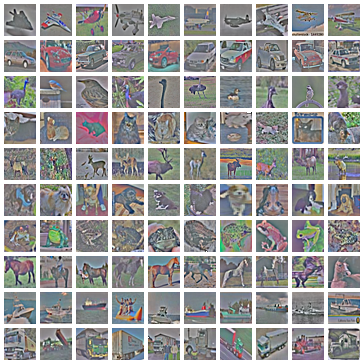
\includegraphics[width=0.5\textwidth]{cifar10zca}
    \caption{Изображения после применения <<ZCA whitening>> с параметром $\alpha=0,1$}
\end{figure}
Предобработка с помощью <<ZCA whitening>> уменьшила ошибку в среднем на $1,5\%$. Кроме того, каждое изображение было
увеличено до 40$\times$40 пикселей, для того чтобы в процессе обучения вырезать из 
изображения случайный патч размером 32$\times$32. Такой приём позволяет снизить эффект переобучения модели и повысить конечную 
точность распознавания.

\subsection{Обучение нейронных сетей}
Походу исследования были проверены различные гипотезы, архитектуры и эвристики так или иначе влияющие на конечные точности 
моделей. В результате различных экспериментов были отобраны семь нейронных сетей, показавшие наилучший результат на тестировании.
Далее будут описаны каждая из отобранных сетей, их свойства и особенности обучения.

\subsubsection{Модель I}
Модель I имеет самую низкую ошибку в предсказаниях среди всех обученных моделей ($6,7\%$). СНН состоит из 18 обучающихся слоёв.
Всего в нейронной сети $\approx2,7$ млн. параметров. Архитектура сети отражена в таблице~\ref{models-table}.

Maxout в качестве функции активации является её отличительной особенностью.
На рисунке~\ref{fig:model_I_maxout_example} показано как maxout соединён с выходами свёрточных слоёв. На
рисунке~\ref{fig:model_I_maxout_ip_example} можно видеть соединение выходов полносвязного слоя и активации.
Также, после каждого <<пулинг>> (pooling) слоя расположен <<дропаут>> (dropout) с параметром 0,2, который помогает
снизить эффект переобучения сети.
\begin{figure}[h]
    \centering
    \begin{subfigure}[b]{0.5\textwidth}
        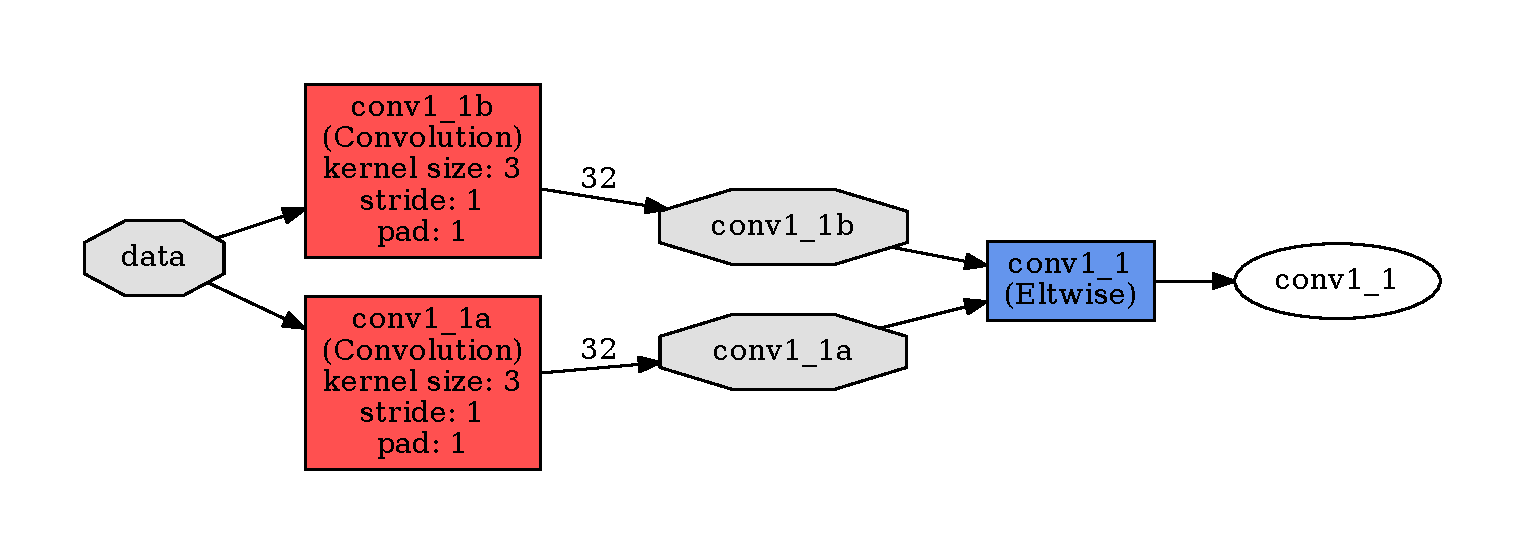
\includegraphics[width=\textwidth]{model_I_maxout_example}
        \vspace*{0.13cm}
        \subcaption{}
        \label{fig:model_I_maxout_example}
    \end{subfigure}~
    \begin{subfigure}[b]{0.5\textwidth}
        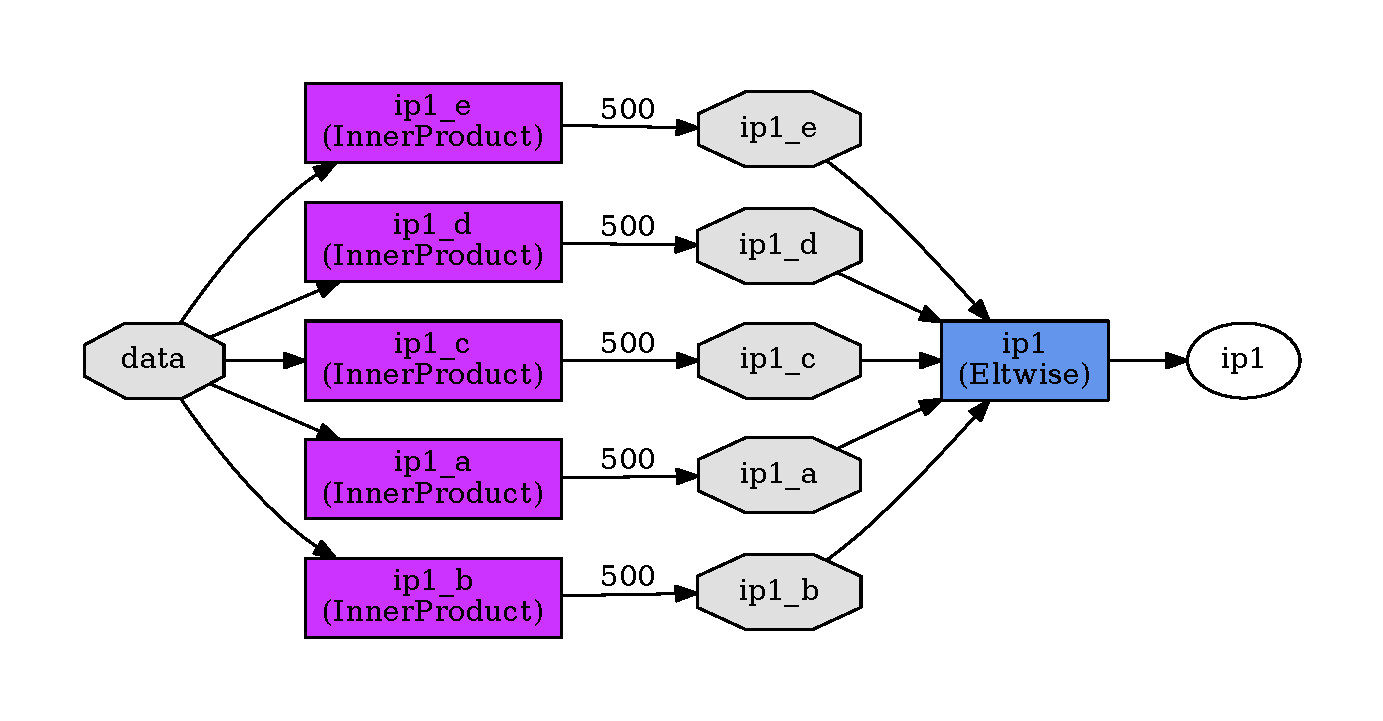
\includegraphics[width=\textwidth]{model_I_maxout_ip_example}
        \subcaption{}
        \label{fig:model_I_maxout_ip_example}
    \end{subfigure}
    \caption{Пример соединения maxout активаций в Модели I}
    \label{fig:maxout_model_I}
\end{figure}

Нейронная сеть обучалась 90\,000 итераций методом стохастического градиентного спуска с моментом (stochastic gradient descent with momentum),
с начальным learning rate (lr) 0,01 и моментом 0.9. Кроме того, использовалась L2 регуляризация с коэффициентом 0,0005.
В процессе обучения, начиная с 40\,000 итерации, lr уменьшался в десять раз каждые 20\,000 итераций.
Таким образом, к концу обучения lr достиг значения $10^{-5}$. Mini batch состоял из 256 изображений. Графики обучения представлены
на рисунке \ref{fig:model_I_pipeline}.

\begin{figure}[H]
    \centering
    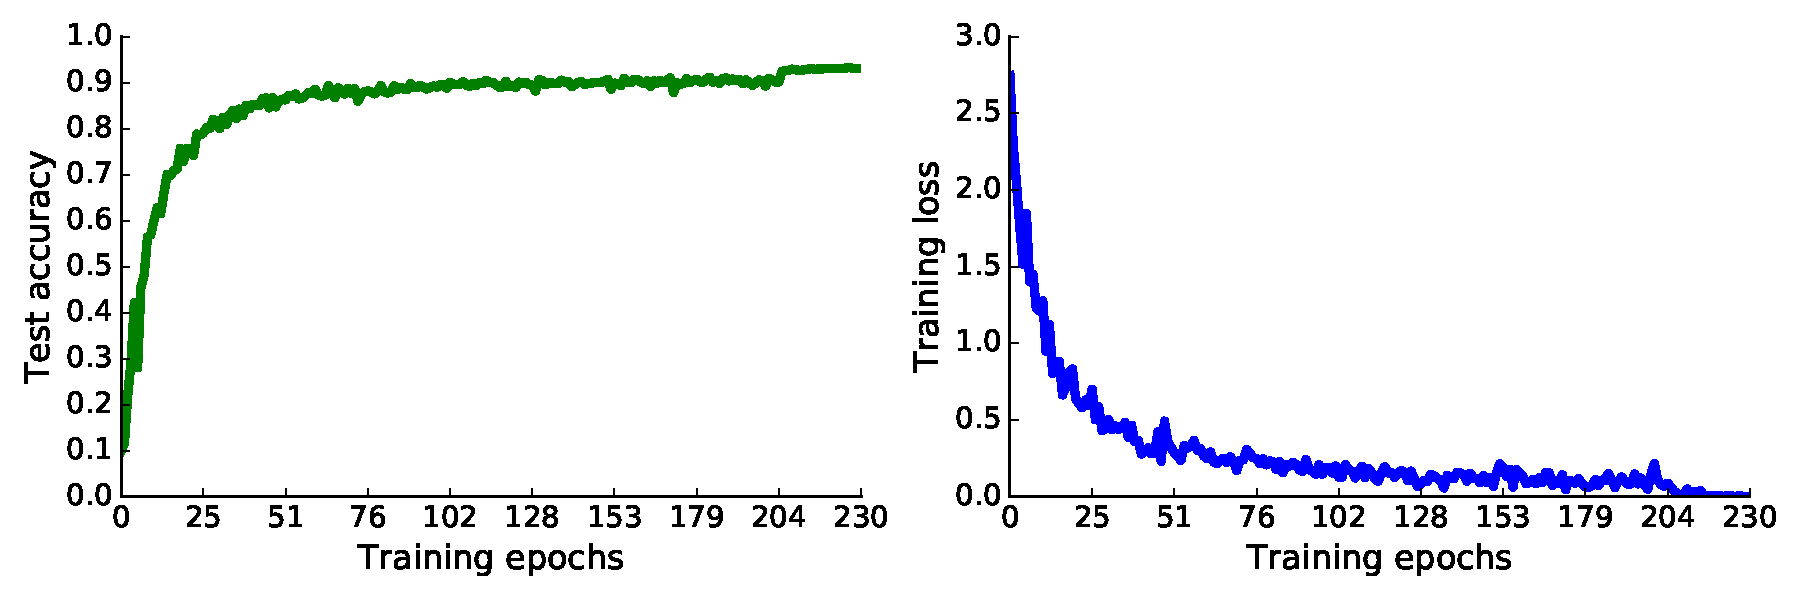
\includegraphics[width=0.9\textwidth]{model_I_pipeline}
    \caption{Графики изменения точности и ошибки в процессе обучения Модели~I}
    \label{fig:model_I_pipeline}
\end{figure}

\subsubsection{Модель II}
Модель II имеет в 4,5 раза меньше параметров, чем Модель I. Их число составляет $\approx600$ тысяч.
Данная нейронная сеть имеет классическую архитектуру, --- чередование свёрточных и <<пулинг>> слоёв, в качестве
функции активации используется Leaky ReLU\footnote{$f(x) = \max(x, \alpha x)$} с параметром $\alpha = 0,01$.
\subsection{Анализ результатов одиночных моделей}
\subsection{Объединение нейронных сетей в ансамбль}